% Basic preamble
\documentclass[Afour,sageh,times]{includes/tex/sagej}

% Pull from header includes
% sage_latex_guidelines.tex V1.20, 14 January 2017
\usepackage{moreverb,url}
\usepackage[colorlinks,bookmarksopen,bookmarksnumbered,citecolor=red,urlcolor=red]{hyperref}
\usepackage{xcolor}
\usepackage{tipa}

% Allow syntax highlighting for r code
\usepackage{color}
\usepackage{fancyvrb}
\newcommand{\VerbBar}{|}
\newcommand{\VERB}{\Verb[commandchars=\\\{\}]}
\DefineVerbatimEnvironment{Highlighting}{Verbatim}{commandchars=\\\{\}}
% Add ',fontsize=\small' for more characters per line
\usepackage{framed}
\definecolor{shadecolor}{RGB}{248,248,248}
\newenvironment{Shaded}{\begin{snugshade}}{\end{snugshade}}
\newcommand{\KeywordTok}[1]{\textcolor[rgb]{0.13,0.29,0.53}{\textbf{#1}}}
\newcommand{\DataTypeTok}[1]{\textcolor[rgb]{0.13,0.29,0.53}{#1}}
\newcommand{\DecValTok}[1]{\textcolor[rgb]{0.00,0.00,0.81}{#1}}
\newcommand{\BaseNTok}[1]{\textcolor[rgb]{0.00,0.00,0.81}{#1}}
\newcommand{\FloatTok}[1]{\textcolor[rgb]{0.00,0.00,0.81}{#1}}
\newcommand{\ConstantTok}[1]{\textcolor[rgb]{0.00,0.00,0.00}{#1}}
\newcommand{\CharTok}[1]{\textcolor[rgb]{0.31,0.60,0.02}{#1}}
\newcommand{\SpecialCharTok}[1]{\textcolor[rgb]{0.00,0.00,0.00}{#1}}
\newcommand{\StringTok}[1]{\textcolor[rgb]{0.31,0.60,0.02}{#1}}
\newcommand{\VerbatimStringTok}[1]{\textcolor[rgb]{0.31,0.60,0.02}{#1}}
\newcommand{\SpecialStringTok}[1]{\textcolor[rgb]{0.31,0.60,0.02}{#1}}
\newcommand{\ImportTok}[1]{#1}
\newcommand{\CommentTok}[1]{\textcolor[rgb]{0.56,0.35,0.01}{\textit{#1}}}
\newcommand{\DocumentationTok}[1]{\textcolor[rgb]{0.56,0.35,0.01}{\textbf{\textit{#1}}}}
\newcommand{\AnnotationTok}[1]{\textcolor[rgb]{0.56,0.35,0.01}{\textbf{\textit{#1}}}}
\newcommand{\CommentVarTok}[1]{\textcolor[rgb]{0.56,0.35,0.01}{\textbf{\textit{#1}}}}
\newcommand{\OtherTok}[1]{\textcolor[rgb]{0.56,0.35,0.01}{#1}}
\newcommand{\FunctionTok}[1]{\textcolor[rgb]{0.00,0.00,0.00}{#1}}
\newcommand{\VariableTok}[1]{\textcolor[rgb]{0.00,0.00,0.00}{#1}}
\newcommand{\ControlFlowTok}[1]{\textcolor[rgb]{0.13,0.29,0.53}{\textbf{#1}}}
\newcommand{\OperatorTok}[1]{\textcolor[rgb]{0.81,0.36,0.00}{\textbf{#1}}}
\newcommand{\BuiltInTok}[1]{#1}
\newcommand{\ExtensionTok}[1]{#1}
\newcommand{\PreprocessorTok}[1]{\textcolor[rgb]{0.56,0.35,0.01}{\textit{#1}}}
\newcommand{\AttributeTok}[1]{\textcolor[rgb]{0.77,0.63,0.00}{#1}}
\newcommand{\RegionMarkerTok}[1]{#1}
\newcommand{\InformationTok}[1]{\textcolor[rgb]{0.56,0.35,0.01}{\textbf{\textit{#1}}}}
\newcommand{\WarningTok}[1]{\textcolor[rgb]{0.56,0.35,0.01}{\textbf{\textit{#1}}}}
\newcommand{\AlertTok}[1]{\textcolor[rgb]{0.94,0.16,0.16}{#1}}
\newcommand{\ErrorTok}[1]{\textcolor[rgb]{0.64,0.00,0.00}{\textbf{#1}}}
\newcommand{\NormalTok}[1]{#1}












\begin{document}



% sage_latex_guidelines.tex V1.20, 14 January 2017

\newcommand\BibTeX{{\rmfamily B\kern-.05em \textsc{i\kern-.025em b}\kern-.08em
T\kern-.1667em\lower.7ex\hbox{E}\kern-.125emX}}

\def\volumeyear{2016}


\runninghead{Smith and Wittkopf}

\title{A demonstration of the \LaTeXe\ class file for
\itshape{SAGE Publications}}

\author{Alistair Smith\affilnum{1} and Hendrik Wittkopf\affilnum{2}}

\affiliation{\affilnum{1}Sunrise Setting Ltd, UK\\
\affilnum{2}SAGE Publications Ltd, UK}

\corrauth{Alistair Smith, Sunrise Setting Ltd
Brixham Laboratory,
Freshwater Quarry,
Brixham, Devon,
TQ5~8BA, UK.}

\email{alistair.smith@sunrise-setting.co.uk}

\begin{abstract}
This paper describes the use of the \LaTeXe\
\textsf{\journalclass} class file for setting papers to be
submitted to a \textit{SAGE Publications} journal.
The template can be downloaded \href{http://www.uk.sagepub.com/repository/binaries/SAGE LaTeX template.zip}{here}.
\end{abstract}

\keywords{Class file, \LaTeXe, \textit{SAGE Publications}}

\maketitle


\section{Introduction}

Many authors submitting to research journals use \LaTeXe~to prepare
their papers. This paper describes the \textsf{\journalclass} class file
which can be used to convert articles produced with other \LaTeXe~class
files into the correct form for submission to
\textit{SAGE Publications}.

The \textsf{\journalclass} class file preserves much of the standard
\LaTeXe~ interface so that any document which was produced using the
standard \LaTeXe~ \textsf{article} style can easily be converted to work
with the \textsf{\journalclassshort} style. However, the width of text
and typesize will vary from that of \textsf{article.cls}; therefore,
\textit{line breaks 
will change} and it is likely that displayed mathematics and tabular
material will need re-setting.

In the following sections we describe how to lay out your code to use
\textsf{\journalclass} to reproduce much of the typographical look of
the \textit{SAGE} journal that you wish to submit to. However, this
paper is not a guide to using \LaTeXe~and we would refer you to any of
the many books available
\citep[see, for example,][]{kopka_daly_2003, lamport_1994, mittlebach_goossens_2004}

\section{The three golden rules}

Before we proceed, we would like to stress \textit{three golden rules}
that need to be followed to enable the most efficient use of your code
at the typesetting stage:

\begin{enumerate}
  \item[(i)] keep your own macros to an absolute minimum;
  \item[(ii)] as \TeX\ is designed to make sensible spacing decisions by 
  itself, do \textit{not} use explicit horizontal or vertical spacing 
  commands, except in a few accepted (mostly mathematical) situations, such as 
  \verb"\," before a differential~d, or \verb"\quad" to separate an equation 
  from its qualifier;
  \item[(iii)] follow the journal reference style.
\end{enumerate}

\section{Getting started}

The \textsf{\journalclassshort} class file should run on any standard
\LaTeXe~ installation. If any of the fonts, style files or packages it
requires are missing from your installation, they can be found on the
\textit{\TeX\ Collection} DVDs or downloaded from CTAN.

\begin{figure*}
  \setlength{\fboxsep}{0pt}%
  \setlength{\fboxrule}{0pt}%
  \begin{center}
  \begin{verbatim}
  \documentclass[<options>]{sagej}

  \begin{document}

  \runninghead{<Author surnames>}

  \title{<Initial capital only>}

  \author{<An Author\affilnum{1},
  Someone Else\affilnum{2} and
  Perhaps Another\affilnum{1}>}

  \affiliation{<\affilnum{1}First and third authors' affiliation\\
  \affilnum{2}Second author affiliation>}

  \corrauth{<Corresponding author's name and full postal address>}

  \email{<Corresponding author's email address>}

  \begin{abstract}
  <Text>
  \end{abstract}

  \keywords{<List keywords>}

  \maketitle

  \section{Introduction}
  .
  .
  .
  \end{verbatim}
  \end{center}
  \caption{Example header text.\label{F1}}
\end{figure*}

\section{The article header information}

The heading for any file using \textsf{\journalclass} is shown in Figure
\ref{F1}. You must select options for the trim/text area and the
reference style of the journal you are submitting to. The choice of
\verb+options+ are listed in Table \ref{T1}.

\begin{table}[h]
  \small\sf\centering
  \caption{The choice of options.\label{T1}}
  \begin{tabular}{lll}
  \toprule
  Option              & Trim and font size         & Columns       \\
  \midrule
  \texttt{shortAfour} & 210 $\times$ 280 mm, 10pt  & Double column \\
  \texttt{Afour}      & 210 $\times$ 297 mm, 10pt  & Double column \\
  \texttt{MCfour}     & 189 $\times$ 246 mm, 10pt  & Double column \\
  \texttt{PCfour}     & 170 $\times$ 242 mm, 10pt  & Double column \\
  \texttt{Royal}      & 156 $\times$ 234 mm, 10pt  & Single column \\
  \texttt{Crown}      & 7.25 $\times$ 9.5 in, 10pt & Single column \\
  \texttt{Review}     & 156 $\times$ 234 mm, 12pt  & Single column \\
  \bottomrule
  \end{tabular}\\[10pt]
  \begin{tabular}{ll}
  \toprule
  Option&Reference style\\
  \midrule
  \texttt{sageh}&SAGE Harvard style (author-year)\\
  \texttt{sagev}&SAGE Vancouver style (superscript numbers)\\
  \texttt{sageapa}&APA style (author-year)\\
  \bottomrule
  \end{tabular}
\end{table}

For example, if your journal is short A4 sized, uses Times fonts and has
Harvard style references then you would need

\begin{small}
\noindent \verb+\documentclass[ShortAfour,times,sageh]{sagej}+
\end{small}

Most \textit{SAGE} journals are published using Times fonts but if for
any reason you have a problem using Times you can easily resort to
Computer Modern fonts by removing the \verb"times" option.

\subsection{'Review' option}

Some journals (for example,
\emph{Journal of the Society for Clinical Trials}) require that papers
are set single column and with a larger font size to help with the
review process. If this is a requirement for the journal that you are
submitting to, just add the \verb+Review+ option to the
\verb+\documenclass[]{sagej}+ line.

\subsection{Remarks}

\begin{enumerate}
  \item[(i)] In \verb"\runninghead" use `\textit{et~al.}' if there are three 
  or more authors.
  \item[(ii)] For multiple author papers please note the use of 
  \verb"\affilnum" to link names and affiliations. The corresponding author 
  details need to be included using the \verb+\corrauth+ and 
  \verb+\email+ commands.
  \item[(iii)] For submitting a double-spaced manuscript, add 
  \verb"doublespace" as an option to the documentclass line.
  \item[(iv)] The abstract should be capable of standing by itself, in the 
  absence of the body of the article and of the bibliography. Therefore, it 
  must not contain any reference citations.
  \item[(v)] Keywords are separated by commas.
  \item[(vi)] If you are submitting to a \textit{SAGE} journal that requires 
  numbered sections (for example, IJRR), please add the command 
  \verb+\setcounter{secnumdepth}{3}+ just above the \verb+\begin{document}+ 
  line.
\end{enumerate}

\section{The body of the article}

\subsection{Mathematics}

\textsf{\journalclass} makes the full functionality of
\AmS/\TeX~available. We encourage the use of the \verb"align",
\verb"gather" and \verb"multline" environments for displayed
mathematics. \textsf{amsthm} is used for setting theorem-like and proof
environments. The usual \verb"\newtheorem"command needs to be used to
set up the environments for your particular document.

\subsection{Figures and tables}

\textsf{\journalclass} includes the \textsf{graphicx} package for
handling figures.

Figures are called in as follows:

\begin{verbatim}
\begin{figure}
\centering
\includegraphics{<figure name>}
\caption{<Figure caption>}
\end{figure}
\end{verbatim}

For further details on how to size figures, etc., with the
\textsf{graphicx} package see, for example, \cite{R1} or \cite{R3}.

The standard coding for a table is shown in Figure \ref{F2}.

\begin{figure}
  \setlength{\fboxsep}{0pt}%
  \setlength{\fboxrule}{0pt}%
  \begin{center}
  \begin{boxedverbatim}
  \begin{table}
  \small\sf\centering
  \caption{<Table caption.>}
  \begin{tabular}{<table alignment>}
  \toprule
  <column headings>\\
  \midrule
  <table entries
  (separated by & as usual)>\\
  <table entries>\\
  .
  .
  .\\
  \bottomrule
  \end{tabular}
  \end{table}
  \end{boxedverbatim}
  \end{center}
  \caption{Example table layout.\label{F2}}
\end{figure}

\subsection{Cross-referencing}

The use of the \LaTeX~cross-reference system for figures, tables,
equations, etc., is encouraged (using \verb"\ref{<name>}" and
\verb"\label{<name>}").

\subsection{End of paper special sections}

Depending on the requirements of the journal that you are submitting to,
there are macros defined to typeset various special sections.

The commands available are:

\begin{verbatim}
  \begin{acks}
  To typeset an
    "Acknowledgements" section.
  \end{acks}
\end{verbatim}

\begin{verbatim}
  \begin{biog}
  To typeset an
    "Author biography" section.
  \end{biog}
\end{verbatim}

\begin{verbatim}
  \begin{biogs}
  To typeset an
    "Author Biographies" section.
  \end{biogs}
\end{verbatim}

\begin{verbatim}
  \begin{dci}
  To typeset a "Declaration of
    conflicting interests" section.
  \end{dci}
\end{verbatim}

\begin{verbatim}
  \begin{funding}
  To typeset a "Funding" section.
  \end{funding}
\end{verbatim}

\begin{verbatim}
  \begin{sm}
  To typeset a
    "Supplemental material" section.
  \end{sm}
\end{verbatim}

\subsection{Endnotes}

Most \textit{SAGE} journals use endnotes rather than footnotes, so any
notes should be coded as \verb+\endnote{<Text>}+. Place the command
\verb+\theendnotes+ just above the Reference section to typeset the
endnotes.

To avoid any confusion for papers that use Vancouver style references,
footnotes/endnotes should be edited into the text.

\subsection{References}

Please note that the files \textsf{SageH.bst} and \textsf{SageV.bst} are
included with the class file for those authors using \BibTeX. The files
work in a completely standard way, and you just need to uncomment one of
the lines in the below example depending on what style you require:

\begin{verbatim}
  %%Harvard (name/date)
  %\bibliographystyle{SageH}
  %%Vancouver (numbered)
  %\bibliographystyle{SageV}
  \bibliography{<YourBibfile.bib>}
\end{verbatim}

\noindent and remember to add the relevant option to the
\verb+\documentclass[]{sagej}+ line as listed in Table \ref{T1}.

\section{Copyright statement}

Please be aware that the use of this \LaTeXe~class file is governed by
the following conditions.

\subsection{Copyright}

Copyright \copyright~\volumeyear~SAGE Publications Ltd, 1 Oliver's Yard,
55 City Road, London, EC1Y\textasciitilde{}1SP, UK. All rights reserved.

\subsection{Rules of use}

This class file is made available for use by authors who wish to prepare
an article for publication in a \textit{SAGE Publications} journal. The
user may not exploit any part of the class file commercially.

This class file is provided on an \textit{as is} basis, without
warranties of any kind, either express or implied, including but not
limited to warranties of title, or implied warranties of
merchantablility or fitness for a particular purpose. There will be no
duty on the author{[}s{]} of the software or SAGE Publications Ltd to
correct any errors or defects in the software. Any statutory rights you
may have remain unaffected by your acceptance of these rules of use.

\section{R}

In this section I show how one can use R and R scripts.

\begin{Shaded}
\begin{Highlighting}[]
\DecValTok{2} \OperatorTok{+}\StringTok{ }\DecValTok{2}
\end{Highlighting}
\end{Shaded}

\begin{verbatim}
## [1] 4
\end{verbatim}

\noindent It is also possible to use inline R code. For example, 2 + 2 =
4. R scripts can be loaded as well:

\begin{Shaded}
\begin{Highlighting}[]
\KeywordTok{source}\NormalTok{(}\StringTok{"./includes/scripts/analysis.R"}\NormalTok{)}
\end{Highlighting}
\end{Shaded}

\noindent Which means you have access to any objects assigned in the
script:

\begin{Shaded}
\begin{Highlighting}[]
\NormalTok{cars_plot}
\end{Highlighting}
\end{Shaded}

\begin{flushleft}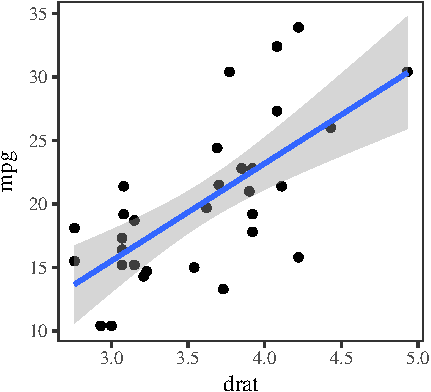
\includegraphics{./includes/figs/ex_plot-1} \end{flushleft}

\begin{acks}
This class file was developed by Sunrise Setting Ltd, Brixham, Devon, UK. \\
Website: \url{http://www.sunrise-setting.co.uk}
\end{acks}

\bibliographystyle{./includes/bib/SageH}\bibliography{./includes/bib/example.bib}


\end{document}
